\subsection{Economic Growth}

\subsubsection{Growth Factors and Production Function}

\begin{remark} \hlt{Preconditions for Economic Growth}
\begin{enumerate}[label=\roman*.]
\setlength{\itemsep}{0pt}
\item Savings and Investment: positively correlated with economic development.\\
For countries to grow, private and public sector investment must provide sufficient level of capital per worker. If insufficient savings, to attract foreign investment in order to grow.
\item Financial Markets and Intermediaries: efficiently allocate resources. Determine projects with best returns of capital on risk-adjusted basis; provide investors with liquidity and opportunities for risk reduction; pool savings to finance projects on larger scales than otherwise possible. However, intermediation may lead to declining credit standards, increases in leverage, increasing risk but not economic growth.
\item Political Stability, Rule of Law, Property Rights: countries with developed system of property rights will attract capital. Economic uncertainty caused by wars, corruption, disruptions creates unacceptable risk, reducing potential economic growth.
\item Investment in Human Capital: complementary to growth in physical capital, result in higher growth rates. Developed countries benefit the most from post-secondary education spending, which foster innovation. Less-developed countries benefit from spending on primary and secondary education, which enables the workforce to apply the technology developed elsewhere.
\item Tax and Regulatory System: the lower the tax and regulatory burden, the higher the rate of economic growth. Lower regulation foster entrepreneurial activity which increases productivity.
\item Free Trade and Unrestricted Capital Flows: promotes growth by providing competition for domestic firms, increasing overall efficiency and reducing costs. Opens up new markets for domestic producers. Mitigates issue of insufficient domestic savings as foreign capital may increase capital, invested directly in property, physical plant and equipment (FDI), or invested indirectly in financial assets.
\end{enumerate}
\end{remark}

\begin{remark} \hlt{Equity Prices and Potential GDP}\\
Aggregate corporate earnings can grow if GDP grows or if share of corporate earnings in GDP grows.\\
Share of corporate profits in GDP cannot increase indefinitely as labour will be unwilling to work for lower proportion of GDP. Hence potential GDP is the long-run limit of earnings growth.
\end{remark}

\begin{definition} \hlt{Grinold-Kroner Decomposition}\\
Captures relationship between equity returns and economic growth.
\begin{align}
E(R_e) &= \text{Dividend Yield} + \text{Expected Capital Gain} \nonumber \\
&= \text{Dividend Yield} + \text{Expected Repricing} + \text{Earnings Growth per Share} \nonumber\\
&= dy + \Delta(P/E) + \pi + g - \Delta S \nonumber
\end{align}
where $\Delta (P/E)$ is expected repricing, $\pi$ is inflation rate, $g$ is real economic growth, $\Delta S$ is $\Delta$ shares outstanding.\\
Dividend yield is fairly stable, and is significant contributor to equity market returns.\\
Expected repricing (change in $P/E$) fluctuates with business cycle. When GDP growth is high, market multiples $\uparrow$ as perception of risk $\downarrow$. In long-run, key factor driving equity returns is $g$ (subject to potential GDP growth).\\
Dilution effect ($\Delta S$) impact differs by country depending on its level of development and sophistication of financial markets. The dilution effect is comprised of net stock buybacks ($nbb$) (more appropriately called 'net issuance' $=$ net issuance $-$ buybacks), and issuance held privately by SMEs (relative dynamism, $rd$).
\begin{equation}
\Delta S = nbb + rd \nonumber
\end{equation}
Relative dynamism captures difference between overall economic growth and earnings growth of listed companies
\end{definition}

\begin{remark} \hlt{Potential GDP Growth Effects on Equity and Fixed Income Markets}
\begin{enumerate}[label=\roman*.]
\setlength{\itemsep}{0pt}
\item $\uparrow$ GDP growth $\Rightarrow$ $\uparrow$ equity returns, which are significantly affected by dilution.\\
$\uparrow$ potential GDP growth $\Rightarrow$ future income $\uparrow$ $\Rightarrow$ current consumption $\uparrow$.\\
To encourage consumers to delay consumptions, investments would have to offer higher real rate of return. Hence $\uparrow$ potential GDP growth $\Rightarrow$ $\uparrow$ real interest rates and $\uparrow$ real asset returns.
\item In short term, if actual GDP growth rate $>$ potential GDP growth rate, concerns on inflation increase, central bank more likely to follow restrictive monetary policy. Vice versa for opposite case. \\
Government may run fiscal surplus when actual GDP growth rate $>$ potential GDP growth rate.
\item $\uparrow$ potential GDP growth rate $\Rightarrow$ $\uparrow$ credit quality and $\downarrow$ credit risk.
\end{enumerate}
\end{remark}

\begin{definition} \hlt{Production Function}\\
Let $Y$ be level of aggregate output, $K$ be capital services provided by stock of equipment and structures used to produce goods and services, $L$ is quantity of labour or number of hours worked in economy. Then
\begin{equation}
Y = A \cdot f(K,L) \nonumber
\end{equation}
Note $A$ is \hlt{Total Factor Productivity (TFP)}, the general level of productivity or technology in the economy, from scientific advanced, applied R\&D, improvement in management methods, ways to raise productive capacity.\\
Function may be extended to include raw materials ($N$), human capital ($H$), ICT capital ($K_{IT}$), non-ICT capital ($K_{NT}$), public capital ($K_P$).
\end{definition}

\begin{definition} \hlt{Cobb-Douglas Production Function}\\
Output (GDP) is a function of labour and capital inputs and their productivity.\\
Function exhibits constant returns to scale.
\begin{equation}
 = A \cdot f(K,L) = A \cdot K^{\alpha} L^{(1- \alpha)}, \ \ \ \alpha \in [0,1] \nonumber
\end{equation}
where $\alpha$ is share of output paid by companies to capital and labour.
\end{definition}

\begin{definition} {\color{white}space}
\begin{enumerate}[label=\roman*.]
\setlength{\itemsep}{0pt}
\item Marginal Product of Capital: additional output for one additional unit of $K$
\item Marginal Productivity of Capital: increase in output per worker for one additional unit of $K/L$
\end{enumerate}
Profit maximisation requires marginal product of capital $=$ rental price of capital, marginal product of labour $=$ real wage rate.
\end{definition}

\begin{definition} \hlt{Cobb-Douglas Labour Productivity Measure}\\
Measure is similar to GDP per capita as a standard of living measure.\\
Assuming number of workers and $\alpha$ is constant. Increases in output can be gained by increasing capital per worker $K$ (capital deepening), or improving technology (increases TFP, $A$).
\begin{equation}
\text{Labour Productivity} = \frac{Y}{L} = A \cdot \left( \frac{K}{L} \right)^{\alpha} \nonumber
\end{equation}
Note, as $\alpha < 1$, additional capital has diminishing effect on productivity. $\downarrow \alpha \ \Rightarrow \downarrow$ benefit of capital deepening.\\
Developed markets have high capital-to-labour ratio, hence gains less from capital deepening.
\end{definition}

\begin{figure}[H]
\centering
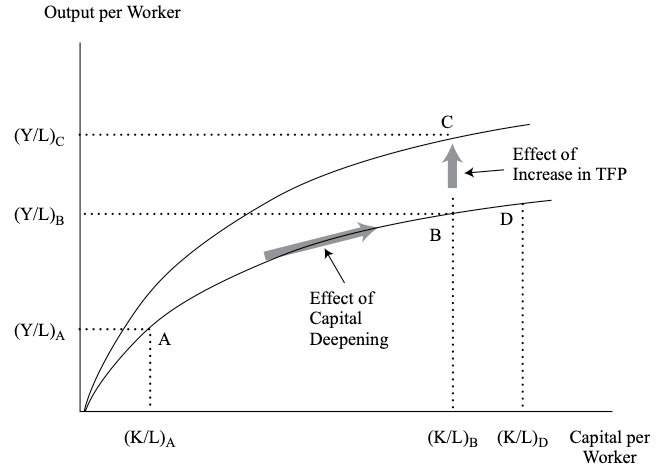
\includegraphics[scale=0.4]{/econ/kdeep}
\caption{Per Capita Production Function Capital Deepening versus Technological (TFP) Progress}
\end{figure}

\begin{remark} \hlt{Capital Deepening versus Technological Progress on Productivity Curve}\\
Capital deepening is movement along productivity curve; curvature derives from diminishing marginal productivity of capital. Economies will increase investment in capital as long as $MPK > r$. At level of $K/L$ for which $MPK = r$, capital deepening stops and labour productivity becomes stagnant.\\
As technological progress occurs, this shifts productivity curve upward as both capital and labour can produce a higher level of output. Developed countries rely on $\uparrow$ TFP for growth in productivity.
\begin{equation}
\text{Labour Productivity Growth Rate} = \text{Growth in $TFP$} + \text{Growth in $K$} \nonumber
\end{equation}
\end{remark}

\begin{remark} \hlt{Steady State Value of $\alpha$}\\
In steady state, marginal product of capital ($MPK = \alpha Y/K$) and marginal cost of capital ($r$) are equal,
\begin{equation}
\alpha = r \frac{K}{Y} \nonumber
\end{equation}
Note, the ratio $rK$ to $Y$ measures output allocated to providers of capital, precisely definition of $\alpha$.
\end{remark}

\begin{definition} \hlt{Growth Accounting Relations}\\
By Cobb-Douglas Production Function, growth in potential GDP can be expressed as
\begin{equation}
\frac{\Delta Y}{Y} = \frac{\Delta A}{A} + \alpha \left( \frac{\Delta K}{K} \right) + (1 - \alpha)\left( \frac{\Delta L}{L} \right) \nonumber
\end{equation}
In practice, levels of capital and labour are forecasted from long-term trends, and shares of capital and labour determined from national income accounts. Change in TFP is not directly observable, estimated as residual.\\
Equation is useful for determining comparative effects of increasing different inputs and estimate potential output.
\end{definition}

\begin{definition} \hlt{Labour Productivity Growth Accounting Equation}\\
Models potential GDP as function of labour input and productivity of labour input.\\
Long-term growth rate in labour productivity reflects both capital deepening and technological progress.
\begin{equation}
\text{Growth rate in potential GDP} = \text{LT labour growth rate} + \text{LT labour productivity growth rate} \nonumber
\end{equation}
\end{definition}

\begin{remark} \hlt{Natural Resources Impact on Economic Growth}
\begin{enumerate}[label=\roman*.]
\setlength{\itemsep}{0pt}
\item Access to natural resources is important, but ownership and production of natural resources is not necessary for a country to achieve high level of income.
\item Ownership of natural resources may actually inhibit growth. Countries rich in natural resources may:
\begin{enumerate}[label=\arabic*.]
\setlength{\itemsep}{0pt}
\item fail to develop economic institutions necessary for growth
\item suffer from 'Dutch disease', where currency appreciation driven by strong export demand for resources make other segments of economy globally uncompetitive
\end{enumerate}
Non-renewable natural resources will eventually limit growth, as rapid economic growth will cause resource depletion. TFP will make resource usage efficient. Growing scarcity of specific resources will increase their price, encourage a shift towards more plentiful substitutes. Share of national income going to land and resources declining as composition of output shifts more towards services.
\end{enumerate}
\end{remark}

\begin{remark} \hlt{Labour Supply Factors}
\begin{enumerate}[label=\roman*.]
\setlength{\itemsep}{0pt}
\item Demographics: long-term projections of labour supply determined by growth of working age population via fertility and mortality rates. Population growth may increase growth rate of economy, but no impact on rate of increase per capita GDP. Age mix is also important; younger population joining is a boost.
\item Labour Force Participation: an increase in participation rate may raise growth of per capita GDP. Changes in participation is a transition to newer/higher level of participation, not permanent rate of change.
\begin{equation}
\text{Labour Force Participation} = \frac{\text{Labour Force}}{\text{Working Age Population}} \nonumber
\end{equation}
\item Immigration: increase migration is solution to slowing labour force growth.
\item Averaged Hours Worked: highly sensitive to business cycle. Long-term average is towards a shorter work week in advanced countries due to legislation, collective bargaining agreements, growth of part-time and temporary work, ‘wealth effect’, high tax rates in labour income.
\end{enumerate}
\end{remark}

\begin{remark} \hlt{Investment in Human Capital on Economic Growth}\\
Human capital is accumulated knowledge, skills that workers acquire from education, training, life experience.\\
Better-educated and more-skilled workers are more productive, more adaptable to changes in technology or other shifts in market demand and supply, and may innovate (external spillover effects).\\
Increased through investment in education and on-the-job training.
\end{remark}

\begin{remark} \hlt{Investment in Public Infrastructure on Economic Growth}\\
Complements the production of private goods and services.\\
Full impact extend beyond direct benefits of the projects, boosting private investment productivity.
\end{remark}

\begin{remark} \hlt{Investment in Physical Capital on Economic Growth}\\
Increases as long as net investment is positive, hence results in higher rate of GDP growth.\\
Generally separated into infrastructure, computers, telecommunications capital (ICT), and non-ICT capital.\\
Actual impact depends on capital-to-labour ratio.\\
Even though LT sustainable growth cannot rely on pure capital deepening, there is strong correlation between investment spending and economic growth as:
\begin{enumerate}[label=\roman*.]
\setlength{\itemsep}{0pt}
\item investment-driven growth lasts for considerable period for countries with relatively low levels of $K/L$
\item impact of investment spending on available capital depends on existing physical stock. If low level of physical stock initially, then impact will be significant.
\item physical capital is not homogeneous. Composition of investment spending and stock of physical capital matters for growth and productivity. Capital spending may be separated into ICT and non-ICT spending.
\begin{enumerate}[label=\arabic*.]
\setlength{\itemsep}{0pt}
\item ICT Spending: growth in IT caused price of key technologies to fall dramatically, increase rate of economic and productivity growth. Produces network externalities; the more people in the network, the greater the potential productivity gains; captured in TFP effect.
\item Non-ICT Spending: non-residential construction, transport equipment, machinery. Result in capital deepening, hence less impact on potential GDP growth.
\end{enumerate}
\end{enumerate}
\end{remark}

\begin{remark} \hlt{Investment in Technology on Economic Growth}\\
Allows overcoming of diminishing marginal returns, results in upward shift in production function.\\
Produce more and higher-quality goods and services with the same resources or inputs.\\
Embodied in human capital and/or in new machinery, equipment and software. Innovate through R\&D.
\end{remark}

\subsubsection{Theories of Growth}

\begin{definition} \hlt{Classical (Malthusian) Theory of Growth}\\
Population growth with limited resources. Production function only has labour input, and land is fixed.\\
$\uparrow$ capital or technological progress $\Rightarrow$ $\uparrow$ per capita income above subsistence level $\Rightarrow$ $\uparrow$ population growth.\\
In long run, new technology results in larger but not richer population.\\
Model is not supported by empirical evidence:
\begin{enumerate}[label=\roman*.]
\setlength{\itemsep}{0pt}
\item as growth per capital income increase, population growth slowed
\item growth per capital income possible as tech progress $>$ diminishing marginal return
\end{enumerate}
\end{definition}

\begin{figure}[H]
\centering
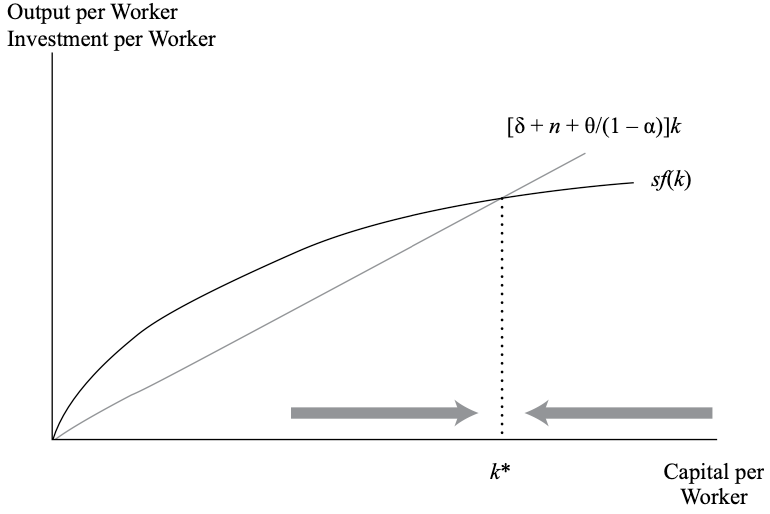
\includegraphics[scale=0.32]{/econ/neoclasssteady}
\caption{Steady state in neoclassical model}
\end{figure}

\begin{definition} \hlt{Neoclassical (Solow) Theory}\\
To estimate economy's long-term steady-state growth rate, in relation to savings/investment rate, rate of technological change, and population growth. Population growth is independent of economic growth.\\
Economy is at equilibrium when output-to-capital ratio is constant, where $K/L$ and output-per-capita also grow at the equilibrium growth rate $g^{*}$.\\
Let $\theta$ be growth rate in technology, $n$ be growth rate of labour, $s$ be fraction of income saved, $\delta$ be constant depreciation rate of physical capital stock. The equilibrium output-to-capital ratio is then:
\begin{equation}
\Psi = \frac{Y}{K} = \left(\frac{1}{s} \right) \left[ \left( \frac{\theta}{1-\alpha} \right) + \delta + n \right] \nonumber
\end{equation}
The sustainable growth rates are then
\begin{enumerate}[label=\roman*.]
\setlength{\itemsep}{0pt}
\item Sustainable growth rate of output-per capita $g^* = \frac{\theta}{1-\alpha}$
\item Sustainable growth rate of output $\frac{\Delta Y}{Y} = \frac{\theta}{1-\alpha} + n$
\end{enumerate}
\end{definition}

\begin{figure}[H]
\centering
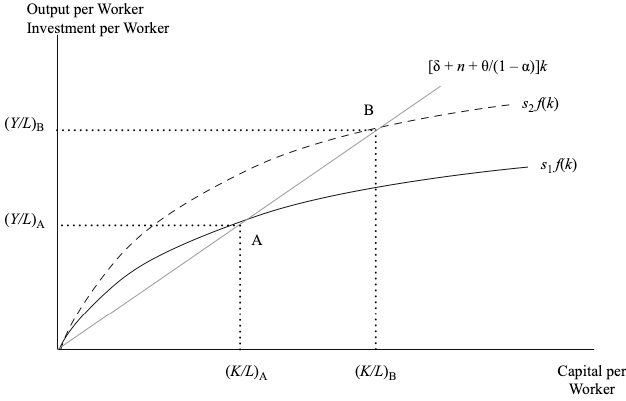
\includegraphics[scale=0.4]{/econ/neoclasssave}
\caption{Impact on Steady State with Increase in $s$}
\end{figure}

\begin{remark} \hlt{Neoclassical Theory: Savings Rate ($s$)}\\
$\uparrow$ savings rate $s$ $\Rightarrow$ $\uparrow$ capital-to-labour ratio $k$ and $\uparrow$ output per worker $y$ as higher savings rate generates more saving/investment at every level of output.\\
The savings/investment curve $sf(k)$ shift upward from initial equilibrium point $A$ to new point $B$, intersecting investment line $[\delta + n + \theta/(1-\alpha)]$ at higher $K/L$ ratios.\\
Note it has not impact on steady growth rates of output per capita or output.
\end{remark}

\begin{figure}[H]
\centering
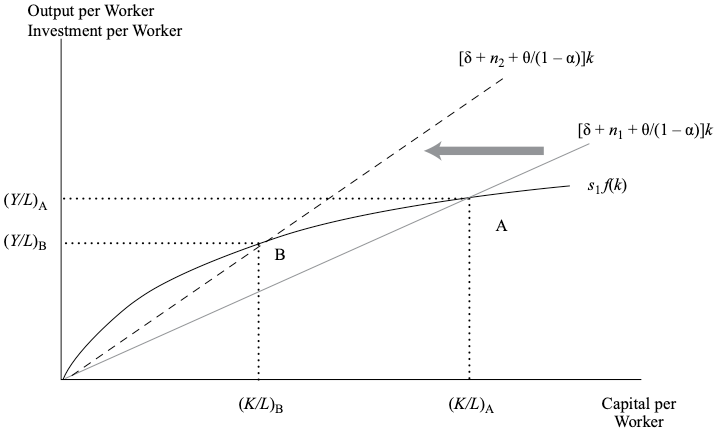
\includegraphics[scale=0.4]{/econ/neoclasslabour}
\caption{Impact on Steady State with Increase in $n, \delta, \theta$}
\end{figure}

\begin{remark} \hlt{Neoclassical Theory: Labour Force Growth Rate ($n$)}\\
$\uparrow$ labour force growth rate $n$ $\Rightarrow$ $\downarrow$ equilibrium capital-to-labour ratio $k$ as a corresponding $\uparrow$ in steady-state growth rate of capital is required. Given gross savings/investment rate, this can be achieved only at a lower capital-to-labour ratio. $\uparrow$ population growth rate $\Rightarrow$ $\uparrow$ slope of required investment line, shifting equilibrium from point $A$ to point $B$, resulting in lower $K/L$ ratios.
\end{remark}

\begin{remark} \hlt{Neoclassical Theory: Depreciation Rate ($\delta$)}\\
$\uparrow$ depreciation rate $\delta$ $\Rightarrow$ $\downarrow$ equilibrium capital-to-labour ratio $k$ as a given rate of gross saving generates less net capital accumulation. Same effect on graph as Labour Force Growth Rate $n$.
\end{remark}

\begin{remark} \hlt{Neoclassical Theory: Growth in TFP ($\theta$)}\\
$\uparrow$ TFP growth rate $\theta$ $\Rightarrow$ $\downarrow$ equilibrium capital-to-labour ratio $k$.\\
$\uparrow$ TFP growth rate $\Rightarrow$ output per worker will grow faster in future, but at fixed point in time, output per worker is lower than it would be with lower $\theta$. Graphically same effect as Labour Force Growth Rate $n$.
\end{remark}

\begin{figure}[H]
\centering
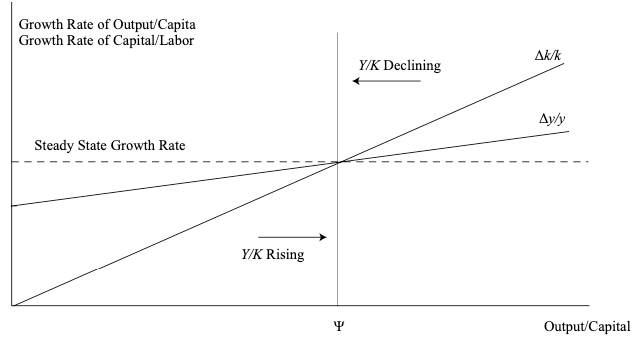
\includegraphics[scale=0.45]{/econ/neoclassdyn}
\caption{Neoclassical Model Dynamics}
\end{figure}

\begin{remark} \hlt{Neoclassical Theory: Transition to Steady State}\\
In transition to steady-state, economy may have faster or slower growth. The growth rates of output-per-capita and capital-to-labour ratio may be written as
\begin{align}
\frac{\Delta y}{y} &= \left( \frac{\delta}{1-\alpha} \right) + \alpha s \left( \frac{Y}{K}  - \Psi \right), \ \ \ \ \ \ \frac{\Delta k}{k} = \left( \frac{\delta}{1-\alpha} \right) + s \left( \frac{Y}{K}  - \Psi \right) \nonumber 
\end{align}
If output-to-capital ratio $Y/K$ $>$ equilibrium level $\Psi$, savings/investment $>$ required investment, above-trend growth in per capita output driven by above-trend rate of capital deepening. Reflect relatively low capital-to-labour ratio, but may also arise from high TFP. As $\alpha < 1$, capital growing faster than output.\\
In long run, growth rates of output per capita and capital-to-labour ratio decline to steady-state.
\end{remark}

\begin{remark} \hlt{Implications of Neoclassical Model}
\begin{enumerate}[label=\roman*.]
\setlength{\itemsep}{0pt}
\item Capital Accumulation
\begin{enumerate}[label=\arabic*.]
\setlength{\itemsep}{0pt}
\item Affects level of output but not growth rate in long-run.
\item Regardless of initial capital-to-labour ratio or level of productivity, a growing economy will move to a point of steady-state growth.
\item Long-run growth $=$ growth rate of labor supply ($n$) $+$ constant growth rate of labor productivity.
\end{enumerate}
\item Capital Deepening vs Technology
\begin{enumerate}[label=\arabic*.]
\setlength{\itemsep}{0pt}
\item Growth $>$ steady-state growth when countries first accumulate capital, but will slow as process of accumulation continues
\item Long-run sustainable growth cannot rely solely on capital deepening investment ($\uparrow K/L$ ratio). If ratio $\uparrow$ too rapidly ($>$ labour productivity), capital becomes less productive, result in slower growth.
\item Increasing supply of some inputs too quickly relative to other inputs lead to diminishing marginal returns; cannot be basis for sustainable growth
\item Without improvements in TFP, $\uparrow$ labour productivity and per capital output would eventually slow
\item Due to diminishing marginal returns to capital, only way to sustain growth in potential GDP per capita is through tech change or growth in TFP. This results in upward shift of production function
\end{enumerate}
\item Convergence
\begin{enumerate}[label=\arabic*.]
\setlength{\itemsep}{0pt}
\item Given relatively scarcity, high marginal productivity of capital and potentially higher savings rates in developing countries, growth rates of developing countries should exceed developed countries
\item Thus there should be convergence of per capital income between developing and developed countries
\end{enumerate}
\item Effect of Savings on Growth
\begin{enumerate}[label=\arabic*.]
\setlength{\itemsep}{0pt}
\item Higher saving rate $s$ $\Rightarrow \downarrow$ steady-state output-to-capital ratio $\Psi$ $\Rightarrow$ $\uparrow$ growth rates of output per capita $y$ and capital-to-labour ratio $k$ above steady-state rate. Growth $>$ steady-state growth rate during transition period. Economy returns to balanced growth thereafter.
\item In transition, economy moves to higher level of per capita output, productivity
\item Once economy achieves steady-state growth, the growth rate does not depend on \% of income saved or invested. Higher savings cannot permanently raise the growth rate of output.
\item Countries with higher savings rates will have higher level of per capita output, higher capital-to-labour ratio, higher labour productivity.
\end{enumerate}
\end{enumerate}
\end{remark}

\begin{definition} \hlt{Endogenous Growth Theory}\\
Technological growth emerges as a result of investment in both physical and human capital.\\
There is no steady state growth rate, so increase in investment can permanently increase the rate of growth.\\
Output per worker is proportional to capital per worker, $y=f(k)=ck$. Output-to-capital ratio is fixed ($=c$).\\
The growth rate of output per capital is 
\begin{equation}
\frac{\Delta y}{y} = \frac{\Delta k}{k} = sc - \delta - n \nonumber
\end{equation}
Note all terms on RHS of equation are constant. Higher savings rate $s$ implies higher growth rate.\\
$\uparrow$ spending on knowledge capital $\Rightarrow$ $\uparrow$ economic growth even in long-run, due to positive externalities.\\
No reason why incomes of developed and developing economies should converge.\\
Externalities associated with knowledge, human capital allow higher-income country to maintain lead.
\end{definition}

\begin{remark} \hlt{Neoclassical versus Endogenous Growth Theory}\\
Neoclassical theory assumes that capital investment will expand as technology improves (i.e., growth comes from increases in TFP not related to the investment in capital).\\
Endogenous growth theory assumes capital investment improve total factor productivity.
\end{remark}

\begin{figure}[H]
\centering
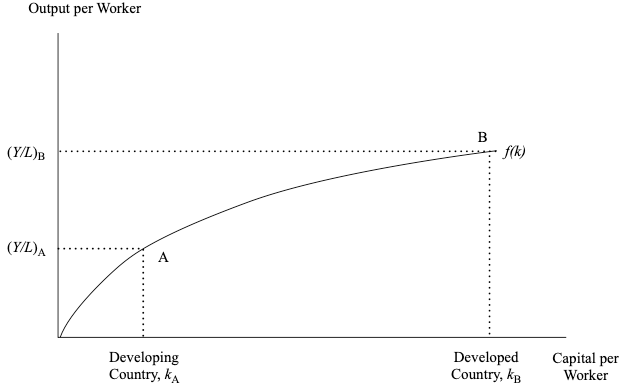
\includegraphics[scale=0.4]{/econ/developedvsdeveloping}
\caption{Per Capita Production Function Developed versus Developing Countries}
\end{figure}

\begin{definition} \hlt{Absolute Convergence}\\
Developing countries will catchup with developed countries and match in per capita output.\\
Neoclassical model assumes all countries have same tech access. Implies convergence of per capita growth rates; do not imply level of per capita income will be same, hence no absolute convergence.
\end{definition}

\begin{definition} \hlt{Conditional Convergence}\\
Convergence conditional on countries with same savings rate, population growth rate, production function.\\
Neoclassical model implies convergence to same level of per capita output and steady-state growth rate.
\end{definition}

\begin{definition} \hlt{Club Convergence}\\
Only rich and middle-income countries that are members of the club are converging to income level of richest countries. Poor countries may join the club if they make appropriate institutional changes.\\
Countries in the club with lower per capita income should provide higher rate of return than investing in higher income countries, with higher risk also.
\end{definition}

\begin{definition} \hlt{Non-Convergence Trap}\\
Countries do not implement necessary institutional reforms. Certain institutional arrangements that initially enhance growth may later generate non-convergence traps if maintained too long.
\end{definition}

\begin{remark} \hlt{Convergence of Developed and Developing Countries}\\
Convergence may occur through:
\begin{enumerate}[label=\roman*.]
\setlength{\itemsep}{0pt}
\item Capital accumulation and capital deepening
\item Developing countries can imitate or adopt technology already utilised in developed countries; learn scientific and management practices; technology transfers
\end{enumerate}
\end{remark}

\begin{remark} \hlt{Economic Rationales for Government Incentives to Private Investments}\\
Under endogenous growth theory, private sector investments in R\&D and knowledge capital benefit the society by creating externalities; economies may not reach steady state growth but may permanently increase growth by expenditures that provide benefits to both company and society.\\
If externalities are not considered, many R\&D projects do not have expected return high enough to compensate firms for inherence riskiness of R\&D investments. At economy level, resultant level of R\&D investment would be sub-optimal. Government incentives subsidise R\&D investments to increase private spending on R\&D.
\end{remark}

\begin{remark} \hlt{Open Economy Benefits}
\begin{enumerate}[label=\roman*.]
\setlength{\itemsep}{0pt}
\item Country can borrow/lend funds in global markets. Domestic investment can be funded by global savings, hence not constrained by domestic savings.
\item Country can shift resources into industries with comparative advantage
\item Companies access to larger export market, exploit economies of scale, $\uparrow$ reward for successful innovation
\item Countries can import tech, increase rate of tech progress
\item Global trade increases competition, forcing companies to improve
\end{enumerate}
\end{remark}

\begin{remark} \hlt{Neoclassical Model on Open Economy}\\
Open economy increases rate of capital-to-labour ratios convergence. Dynamic adjustment process is:
\begin{enumerate}[label=\roman*.]
\setlength{\itemsep}{0pt}
\item Developing countries have lower capital per worker, hence marginal product of capital is higher. ROI would be higher in developing countries.
\item Capital flow from countries with high ratios to those with low ratios for higher ROI
\item Physical capital stock in developing countries grow more rapidly, even if savings rate is low.\\
$\uparrow$ capital growth $\Rightarrow$ $\uparrow$ productivity growth, causing per capita income to converge
\item Capital inflow matched by offsetting trade flows; capital-poor countries run trade deficit as they borrow globally to finance domestic investment
\item In transition to new steady state, capital inflow temporarily $\uparrow$ rate of growth $>$ steady-state rate of growth
\item Physical capital stock $\uparrow$ $\Rightarrow$ $\downarrow$ ROI. Rate of investment and size of trade deficit $\downarrow$.\\
Growth $\downarrow$ $\Rightarrow$ approach steady-state. If investment $<$ domestic savings, country shift from trade deficit to trade surplus and become an exporter of capital
\item  After reallocation of world savings, there is no permanent increase in rate of growth in economy.\\
Both developed and developing countries converge to steady-rate of growth.
\end{enumerate}
\end{remark}

\begin{remark} \hlt{Endogenous Growth model on Open Economy}\\
More open trade policy will permanently increase rate of economic growth. Global output increased via:
\begin{enumerate}[label=\roman*.]
\setlength{\itemsep}{0pt}
\item Selection effect; increased competition from foreign companies force less efficient domestic firms to exit, more efficient firms to innovate, increasing efficiency
\item Scale effect; producers exploit economies of scale by selling to larger market
\item Backwardness effect: less advanced countries or sectors of economy catching up more advanced countries or sectors via knowledge spill-over
\end{enumerate}
Affects innovation process by encouraging higher levels of spending on R\&D, human capital due to open economy. ROI, economic growth increases.
\end{remark}

\begin{remark} \hlt{Open Economy on Convergence of Standard of Living}\\
As long as countries follow outward oriented policies of integrating their industries with world economy and increasing exports, their standard of living tends to converge to that of more developed economies.\\
Countries following inward-oriented policies and protecting domestic industries can expect slower GDP growth, and convergence may not occur.
\end{remark}